\chapter{Related Work}\label{ch:rel}
\section{Text Classification}

Text Classification is a common supervised learning task in which a body of text, or document containing text, needs to be assigned to a set of class labels. Common applications of text categorization include article categorization, spam detection, sentiment analysis, and authorship attribution \cite{Sebastiani2002, Croft, Shrestha}. Pivotal work in this area includes Joachim’s approach that utilized Support Vector Machines (SVMs), which has remained influential \cite{Joachims1998}. Apart from SVMs, multinomial- and Bernouilli-kernelled Naive Bayes (NB), and Logistic Regression are often utilized for these problems \cite{Croft, Wang2012}. However, in order to enable algorithms to take advantage of the information represented by words, we first need to create a representation of text that algorithms can work with. Common feature-generating methods such as the Bag-of-Words (BoW) model, ngrams, the term frequency-inverse document frequency (tf-idf), and word vectors have been used with great effect \cite{Manning2008}.\\
\\
In the BoW model, originally introduced by Harris \cite{Harris1954} every word gets represented by an index in a vector, which can thus grow incredibly spare with the vocabulary used. A sentence of natural language is then simply represented by a sparse vector containing counts of each word appearing in the vocabulary. A problem is that this vocabulary grows larger the more unique words appear in a text.\\ 
\\
On a conceptual level, ngrams are similar to the BoW approach and can be either applied to words or individual characters. The idea is, to look at adjacent words and take counts of words appearing next to each other, instead of focusing on singular words. For instance, a n-gram approach involving bigrams (2-grams) takes two words together, and produces a feature vector that represents a sentence by these counts. A sliding window approach is used to move across a sentence. Both BoW and ngrams are relatively naive methods of dealing with text, as all words or ngrams are considered to be equally important. \\
\\
The tf-idf weighting method tries to address this problem by multiplying a how often a term appears in a document with a log function of how many documents there are in the collection divided by how many document contain the term. If a word is common across all documents this assigns a lower weight than words that are rare across all documents, meaning that rarer words which are theorized to contribute more to the meaning of a document contribute more. The formula for tf-idf is shown below, where tf is the term frequency of term t in document d, N is the total number of documents in the corpus, and df is the document frequency of term t.
\\
\begin{center}
	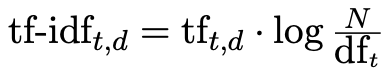
\includegraphics[width=0.35\textwidth]{tf-idf.png}
\end{center}

This has a shortfall in that we still treat words as simply random-ordered features present in a document. Indeed, speakers of natural language will know that word order is actually very important and yet this information is simply lost when converting text to an tf-idf feature vector because it loses the order in which words appear.\\
\\
A different take on word vector representations comes from word embed- dings, popularized by methods such as word2vec \cite{Mikolov2013}. Word embeddings are a representation of a word as a single vector, and the idea has in fact been around for longer \cite{Bengio2003}. These vector space methods often involve a shallow neural network to produce word embeddings learned from processing large amounts of data \cite{Mikolov2013, Levy2014, Goldberg2016}. Commonly, these are 50 to 300-dimensional vectors, although more recent work incorporates much higher dimensionality [\cite{Devlin2018, Peters2018}. As Word2vec was one of the first such methods to become popular, it has been well-studied as a result. The appeal and relative simplicity means it can readily be used for classification, recommendation, and similarity matching \cite{Kenter2015}. Word embedding methods quickly became a state-of-the- art staple in text classification \cite{Peters2018, Howard2018}. However, for classical methods such as SVMs, it appears that using word embeddings decreases performance \cite{Lilleberg2015}.\\
\\
A lot of work has been done to evaluate word embeddings as well to develop new embedding approaches. There many adaptions and similar methods available such as doc2vec \cite{Le2014}, syntax-aware wang2vec \cite{Ling2015}, fastText \cite{Bojanowski2016}, and Stanford’s log bi-linear Glove, which does not rely on a shallow neural network \cite{Pennington2014}.
A key idea is that these embeddings can be learned on data outside the target data set. This is an elegant way to take information from a corpus such as, for instance, a Wikipedia dump and use it to collect contextual information on word occurrences, which can then be applied to, for instance, a sentiment analysis task based on the short text gathered from internet comments. However, the word embeddings learned from data will carry any implicit biases present in their training texts [6], although one could argue this is exactly the type of similarities we intend to capture in the harmonized system text domain. It remains hard to apply word embeddings to scenarios where training data is limited or consisting of short messages. In this line, work has been done to increase performance with data from another domain \cite{Abdelwahab2016}.


\section{Short Text Classification}

A specific sub-field of text categorization deals with short text. Short text is especially prevalent online, where it can take the form of twitter messages, reviews, titles, chat messages, URLs, and search queries. Due to the limited information contained in a message the problem is characterized by data sparsity and a lack of context \cite{Wang2017}. This is especially true with regards to Twitter messages (also known as Tweets) and chat messages, which are often limited in the amount of characters or words in a sentence. Recurring problems are also that these texts do not usually follow natural language conventions: in order to stay brief, these texts often contain a telegram-style syntax and common natural language processing techniques do not apply in the same way they do with spoken text, or longer text as is common in books. This results in a problem of ambiguity, where a piece of text might have multiple meanings but does not provide enough context to figure out which meaning was intended. Often, these texts also include specific tokens and characters unique to the domain. Interestingly, it has been shown that Naive Bayes models outperform SVMs if the text length is limited, while for longer text the opposite still holds true \cite{Wang2012}.

\section{Neural Network for Text}
Neural networks for natural language processing have experienced a surge in popularity in recent years. The most common methods can be roughly grouped in two categories: Convolutional Neural Networks (which includes the approach in this thesis) and Recurrent Neural Networks (which include Long-Short-Term Memory (LSTM) networks and Gated Recurrent Units (GRUs)).\\
\\
Recurrent neural networks are not an odd choice, as they excel with modelling sequential data. They have been utilized for language model problems and have in general been applied with success \cite{Mikolov2010a, Chung2014, Lai2015, Howard2018, Xu}. However, they were initially not well-suited to deal with correlations that are further apart in sentences, due to the vanishing gradient problem during back- propagation where the gradient propagated through the network becomes close to zero when more time steps are made.\\ 
\\
With word embeddings, neural networks for text gained a significant boost in popularity and researchers such as Kim \cite{Kim2014} and Kalchbrenner\cite{Kalchbrenner2014} soon released their work with feed-forward one-dimensional convolutional neural networks based on word embeddings. The general architecture is much simpler than the convolutional neural networks used in computer vision, as the architectures used often consist of just an embedding layer, a convolutional layer, a max-pooling layer and a varying amount of dense layers for each of a set of pre-defined filter sizes. Interestingly, this shallow and wide architecture remains a impressive baseline \cite{Le2017}. The idea behind the convolutional layers’ is that this is akin to taking ngrams with varying convolutional filter sizes \cite{Zhang2015, Jacovi2018} . Pooling strategies have been shown to help, as they eliminate poorer ngrams and bring down the training complexity of the network; however, others opt out of pooling completely [\cite{Kim2014, Zhang2015}. Some architectures use multiple filter sizes in a multi-channel approach \cite{Kim2014,Liu2017,Goldberg2016}.\\
\\
Current approaches also include bi-directional LSTMs, which pass over text both from left-to-right \cite{Radford2018} and right-to-left. This greatly enhances the ability of RNNs to deal with longer dependencies in text. Among these, the ELMo model \cite{Peters2018} successfully applies this concept to produce embeddings that change on differing sentences (context).\\ 


\section{Google BERT}
Attention mechanisms are also popular and are currently popular choices to capture dependencies in text \cite{Lin2017, Openai}. One specific attention mechanism is the transformer, an encoder-decoder architecture that involves an attention mechanism to capture dependencies in text \cite{Vaswani2017}. BERT (Bidirectional Encoder Representations from Transformers) \cite{Devlin2018} successfully combines this idea with a Masked Language Model objective to produce a complex language model that can be applied to many downstream tasks. It is worth noting that the concept of pre-training on outside data and applying a trained model to supervised tasks is still adhered to with these models. However, with these developments it seems that the concept of transfer learning in language models is definitely shifting from mere word embeddings to more sophisticated models that have been trained for a long period of time, which is very much like the trend in computer vision.\\
BERT’s \cite{Devlin2018} (Bidirectional Encoder Representations from Transformers) key technical innovation is applying the bidirectional training of Transformer \cite{Vaswani2017}, a popular attention model, to language modelling. This is a new approach to NLP field which looked at a text sequence either from left to right or combined left-to-right and right-to-left training. The paper’s show that a trained bidirectional language model can have a deeper sense of language context and flow rather than single-direction language models. Researchers also detailed a new technique named MLM (Masked LM) which allows to train bidirectional models which was previously impossible. \\
The model is also pre-trained on two unsupervised tasks, masked language modeling and next sentence prediction. This allows the use of pre-trained BERT model by fine-tuning the same on downstream specific tasks such as sentiment classification, text classification, question answering and more.
\\
In addition to all of that, Google BERT, is the current new standard in NLP algorithm, since he was presented, it has been the new based of many new NLP algorithm such as Facebook RoBERTa \cite{Liu2019d}, XLNet \cite{Yang2019}, Nvidia Megatron \cite{Shoeybi} for exemple. Bert is also mention in other paper \cite{Zhu2019, Wang2019c}. \\ 
\\
Recently Google made a new breakthrough in the NLP field first with ALBERT (A Lite BERT for Self-supervised Learning of Language Representations) \cite{Lan} and a month later with T5\cite{Raffel2019}. ALBERT is using BERT as a based of the new model by tweaking it to make BERT as a lite version and taking off some parameters that are judges as inefficient such as the Next Sentence Prediction (NSP).

\subsection{How Google BERT works ?}
As previously say, BERT,  makes use of Transformer  \cite{Vaswani2017}, an attention mechanism that learns contextual relations between words (or sub-words) in a text. In its vanilla form, Transformer includes two separate mechanisms : 

\begin{itemize}
\item an encoder that reads the text input.
\item a decoder that produces a prediction for the task
\end{itemize}

Since BERT’s goal is to generate a language model, only the encoder mechanism is necessary. This detailed are described in the paper  made by Google researchers \citeauthor{Devlin2018} \cite{Devlin2018}. \\
\\
As opposed to directional models, which read the text input sequentially (left-to-right or right-to-left), the Transformer encoder reads the entire sequence of words at once. Therefore it is considered bidirectional, though it would be more accurate to say that it’s non-directional. This characteristic allows the model to learn the context of a word based on all of its surroundings (left and right of the word).\\
\\
The chart below is a high-level description of the Transformer encoder. The input is a sequence of tokens, which are first embedded into vectors and then processed in the neural network. The output is a sequence of vectors of size H, in which each vector corresponds to an input token with the same index. \\
\\
When training language models, there is a challenge which is to define a prediction goal. Many models predict the next word in a sequence, a directional approach which limits context learning. To overcome this challenge, BERT uses two training strategies:

\begin{itemize}
\item Masked Language Model (MLM)
\item Next Sentence Prediction (NSP)
\end{itemize}

\subsection{Masked Language Model}
Before feeding word sequences into BERT, 15{\%} of the words in each sequence are replaced with a [MASK] token. The model then attempts to predict the original value of the masked words, based on the context provided by the other, non-masked, words in the sequence. In technical terms, the prediction of the output words requires:
\begin{itemize}

\item Adding a classification layer on top of the encoder output.
\item Multiplying the output vectors by the embedding matrix, transforming them into the vocabulary dimension.
\item Calculating the probability of each word in the vocabulary with softmax.
\end{itemize}

\begin{figure}
\centering
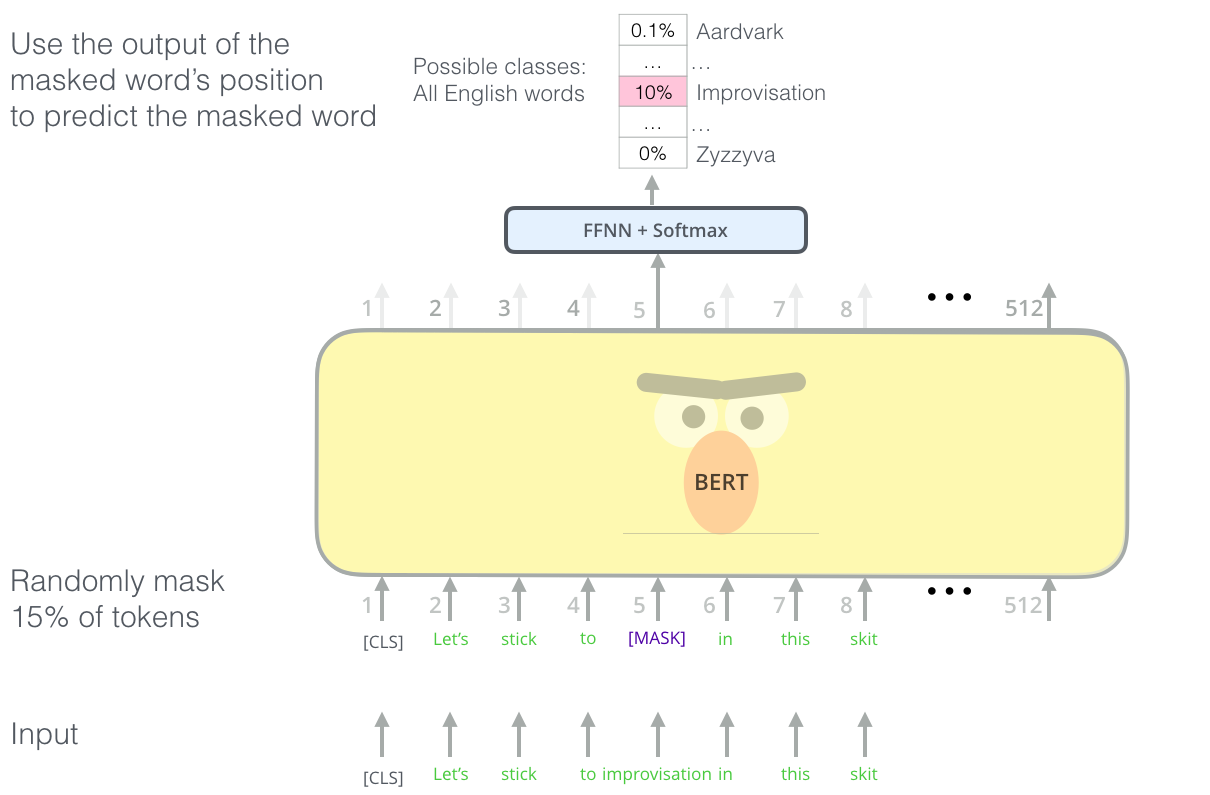
\includegraphics[width=1\textwidth]{BERT-language-modeling-masked-lm.png}
\caption{BERT's clever language modeling task masks 15{\%} of words in the input and asks the model to predict the missing word. \url{https://jalammar.github.io/illustrated-bert/}}
\label{figure 1}
\end{figure}

\chapter{Data Methods}
\section{Data Sets}
\section{Pre-Procession}

\chapter{Methods}
\section{Tokenization for BERT}
\section{Fine-tuning}
